%! Author = Michał_Komputer
%! Date = 14.10.2021

% Preamble
\documentclass[a4paper,11pt]{article}

% Packages
\usepackage[polish]{babel}
\usepackage[T1]{fontenc}
\usepackage[utf8]{inputenc}
\usepackage{array}
\usepackage{enumerate}
\usepackage{float}
\usepackage{graphicx}
\usepackage{latexsym}
\usepackage{polski}
\usepackage{tabularx}
\usepackage[backend=bibtex,style=alphabetic]{biblatex}


% Title page
\title{Praca Inżynierska}
\author{Michał Zawadzki}
\date{Czerwiec 2021}


% Additial settings
\DeclareUnicodeCharacter{266D}{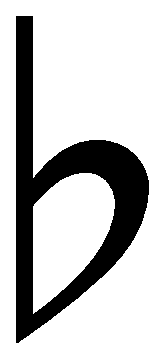
\includegraphics[height=1ex]{music_flat_sign}}
\DeclareUnicodeCharacter{266F}{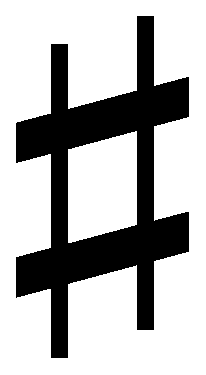
\includegraphics[height=1ex]{music_sharp_sign}}
\addbibresource{references.bib}
\restylefloat{table}

% Document
\begin{document}

    \maketitle

    \tableofcontents


    \section{Wstęp}

    \subsection{Cel pracy}
    Korzystając ze zbioru danych o utworach muzycznych dostępnych na platformie streaming-owej Spotify, stworzono kilka modeli szacujących jaką popularność osiągnie na tej platformie nowy utwór. Modele te są prostymi sieciami neuronowymi o różnej architekturze. Do optymalizacji ich hiper-parametrów uczenia wykorzystano algorytm genetyczny.

    \subsection{Teza główna}
    Algorytm genetyczny może znacząco przyspieszyć proces wyboru optymalnych hiper-parametrów uczenia dla wstępnie zaprojektowanej sieci neuronowej.


    \section{Wpływ cech utworów muzycznych na popularność}

    \subsection{Opis zbioru danych}
    Zbiór danych zawiera informacje o ponad 170 tysiącach utworów muzycznych, opublikowanych w latach 1921-2020 i dostępnych na szwedzkiej platformie streaming-owej Spotify. Dataset został stworzony przy wykorzystaniu oficjalnego, publicznego API deweloperskiego Spotify i udostępniony na platformie Kaggle w formacie CSV przez użytkownika Yamaç Eren Ay.
    \bigskip
    \\ Oryginalny dataset to zbiór tabelaryczny zawierający 170653 rekordów podzielonych na 19 kolumn. Kolumny te to kolejno:
    \begin{itemize}
        \item \textit{valence} (pl.ozdobnik) - Miara w skali od 0.0 do 1.0 określająca stopień 'pozytywności' przekazywany przez utwór. Utwory z wysoką wartością współczynnika \textit{valence} brzmią bardziej pozytywnie (szczęśliwie, radośnie lub euforycznie), podczas gdy niska wartość tego współczynnika objawia się brzmieniem negatywnym (smutnym, depresyjnym, zdenerwowanym lub wściekłym).
        \item \textit{year} (pl. rok) - Rok publikacji utwory. Wartości między 1921 a 2020 włącznie.
        \item \textit{acousticness} (pl. akustyczność) - Miara w skali od 0.0 do 1.0 określająca pewność, z jaką dany utwór można zakwalifikować jako akustyczny. 1.0 - wskazuje na wysoką pewność, 0.0 na bardzo niską.
        \item \textit{artists} (pl. artyści) - Lista imion i nazwisk lub pseudonimów artystycznych artystów wykonujących dany utwór.
        \item \textit{danceability} (pl. taneczność) - Miara w skali od 0.0 do 1.0 określająca, w jakim stopniu dany utwór jest odpowiedni do tańca, wyliczana jako kombinacja takich parametrów muzycznych ja tempo, stabilność rytmu, moc taktu i ogólna regularność. 1.0 oznacza wysoką taneczność, a 0.0 - bardzo niską.
        \item \textit{duration\_ms} (pl. czas trwania) - Czas trwania utworu w milisekundach.
        \item \textit{energy} (pl. energia) - Miara w skali od 0.0 do 1.0 reprezentująca odczuwalny stopień intensywności i aktywności utworu. Typowy utwory 'energetyczne' są odbierane jako szybkie, głośne czy wręcz hałaśliwe. Przykładem wysokiej energetyczności mogą byś utwory death-metalowe, podczas gdy preludia Bacha będą cechowały się niską energetycznością. Postrzegalne czynniki wpływające na tą cechę to dynamiczny zakres, odbierana głośność, tembr, \textit{onset rate} (pl. współczynnik rozpoczęć ??) i ogólna entropia.
        \item \textit{explicit} (pl. odważny, śmiały) - Wartość \textit{true} (pl. prawda)/\textit{false} (pl. fałsz). Flaga określająca czy dany utwór zawiera wulgaryzmy, treści erotyczne, treści nacechowane przemocą, wzmianki o nielegalny używkach i tym podobne; w ogólności treści skierowane do odbiorców pełnoletnich.
        \item \textit{id} (pl. identyfikator) - Unikalne, alfanumeryczne Spotify ID dla utworu.
        \item \textit{instrumentalness} (pl. instrumentalność) - Miara prawdopodobieństwa określająca, czy dany utwór nie zawiera wstawek wokalnych (fragmentów śpiewanych). Wyrazy dźwiękonaśladowcze takie jak 'ooh' czy 'aah' przez algorytm/klasyfikator są traktowane jako instrumentalne. Rap czy zwykła mowa traktowana jako 'czysty wokal'. In bliżej wartości parametru \textit{instrumentalness} do wartości 1.0, tym wyższe prawdopodobieństwo braku wokali. Wartości powyżej 0.5 w założeniu mają reprezentować utwory instrumentalne, natomiast prawdopodobieństwo prawidłowej klasyfikacji rośnie wraz ze zbliżaniem się wskaźnika do wartości 1.0.
        \item \textit{key} (pl. tonacja). Tonacja utworu przedstawiona jako liczba całkowita nieujemna: 0,1,2\ldots . Liczby zmapowane są na standardową notację muzyczną: 0 = C, 1 = C♯/D♭, 2 = D i tak dalej.
        \item \textit{liveness} - (pl. żywość, żywiołowość) - Miara żywiołowości określa prawdopodobieństwo obecność publiczności podczas nagrania. Wartości \textit{liveness} powyżej 0.8 wskazują na wysokie prawdopodobieństwo, że utwór wykonywany był 'na żywo'.
        \item \textit{loudness} (pl. głośność) - Ogólna głośność utworu mierzona w decybelach. Wartości głośności są wyliczane poprzez uśrednienie głośności całego utworu, co sprawia, że metryka staje się użyteczna do porównywania utworów. Głośność jest cechą dźwięku ściśle skorelowaną z amplitudą fali dźwiękowej. Wartości w większości przypadków wahają się między -60 a 0 db.
        \item \textit{mode} (pl. tryb, dominanta) - Parametr 'mode' oznacza modalność utworu: \textit{major} (pl. główna, pierwszoszędna) lub \textit{minor} (pl. pomniejsza, drugorzędna), w znaczeniu typu skali, w której znajduje się warstwa melodyczna. 1 oznacza \textit{major}, 0 to \textit{minor}.
        \item \textit{name} (pl. nazwa) - Tytuł piosenki, utworu lub nagrania.
        \item \textit{popularity} (pl. popularność) - Popularność utworu w skali od 0 do 100, gdzie 100 oznacza najwyższą popularność. Popularność wyliczana jest przez algorytm, bazujący przede wszystkim na liczbie odtworzeń utworu, ale także na tym jak świeże (odległe od chwili obecnej) są te odtworzenia.
        \item \textit{release\_date} (pl. data publikacji) - Data publikacji utworu lub albumu, na którym znalazł się utwór.
        \item \textit{speechiness} (pl. wypełnienie mową) - Parametr \textit{speechiness} określa stopień obecności mowy w utworze. Nagrania wypełnione mową takie jak programy 'talk show', audiobooki czy poematy będą uzyskiwały wartości tego parametru zbliżone do 1.0. Wartości powyżej 0.66 wskazują na wysokie prawdopodobieństwo wypełnienia nagrania w całości mową. Wartości od 0.33 do 0.66 wskazują na występowanie zarówno mowy jak i muzyki, zarówno w następujących po sobie sekwencjach, jak i w nakładających się na siebie wastwach dźwiękowych. Wartości poniżej 0.33 oznaczają duże prawdopodobieńswto nie występowania mowy w utworze.
        \item \textit{tempo} (pl. tempo) - Ogólne szacowane tempo utworu w taktach na minutę (ang. \textit{BPM}). W terminologi muzycznej, tempo jest szybkością danego fragmentu/kawałka utworu wyliczną bezpośrednio w oparciu o średnią długość taktu.
    \end{itemize}
    Opisy parametrów są luźnym tłumaczeniem oficjalnej dokumentacji API deweloperskiego Spotify\cite{SpotifyWebAPIReference}.
    \bigskip
    \\ Do stworzenia modeli wykorzystano następujące parametry: \textit{valence}, \textit{acousticness}, \textit{danceability}, \textit{duration\_ms}, \textit{energy}, \textit{explicit}, \textit{instrumentalness}, \textit{key}, \textit{liveness}, \textit{loudness}, \textit{mode}, \textit{release\_date}, \textit{speechiness} i \textit{tempo} Trzeba tu nadmienić, że na potrzeby dalszych działań wartości parametru \textit{key} zostały zamienione na binarną postać wektorową (ang. \textit{one-hot encoding}), a wartości \textit{release\_date} na milisekundy w standardzie UNIX. Na podstawie wartości wcześniej wymienionych parametrów modele szacowały wartość popularności (ang. \textit{popularity}) utworu.


    \section{Sieci neuronowe}


    \section{Algorytmy Genetyczne}


    \section{Zastosowanie dwustopniowego algorytmu uczenia maszynowego do predykcji popularności utworu}


    \section{Rezultaty eksperymentów}


    \section{Wnioski}


    \printbibliography
\end{document}